\mfpicnumber{1}

\opengraphsfile{GraphsofPolynomials}

\setcounter{footnote}{0}

\label{GraphsofPolynomials}

Three of the families of functions studied thus far -- constant, linear and  quadratic -- belong to a much larger group of functions called \textbf{polynomials}.  We begin our formal study of general polynomials with a definition and some examples.

\smallskip

\colorbox{ResultColor}{\bbm

\begin{defn} \label{polynomialfunction} A \index{function ! polynomial}\index{polynomial function ! definition of}\textbf{polynomial function} is a function of the form \[ f(x) = a_{n} x^{n} + a_{n-\mbox{\tiny$1$}} x^{n-\mbox{\tiny$1$}} + \ldots + a_{\mbox{\tiny $2$}} x^{\mbox{\tiny $2$}} + a_{\mbox{\tiny $1$}} x + a_{\mbox{\tiny $0$}},\] where $a_{\mbox{\tiny $0$}}$, $a_{\mbox{\tiny $1$}}$, \ldots, $a_{n}$ are real numbers and $n \geq 1$ is a natural number.  The domain of a polynomial function is $(-\infty, \infty)$.

\end{defn}

\ebm}

\medskip

There are several things about Definition \ref{polynomialfunction} that may be off-putting or downright frightening.  The best thing to do is look at an example.  Consider $f(x) = 4x^5 - 3x^2 + 2x - 5$.  Is this a polynomial function?  We can re-write the formula for $f$ as $f(x)= 4x^5 + 0 x^{4} + 0 x^{3} + (-3)x^2 + 2 x + (-5).$  Comparing this with Definition \ref{polynomialfunction}, we identify $n=5$, $a_{\mbox{\tiny $5$}} = 4$, $a_{\mbox{\tiny $4$}} = 0$, $a_{\mbox{\tiny $3$}} = 0$, $a_{\mbox{\tiny $2$}} = -3$, $a_{\mbox{\tiny $1$}} = 2$ and $a_{\mbox{\tiny $0$}} = -5$.  In other words, $a_{\mbox{\tiny $5$}}$ is the coefficient of $x^{5}$, $a_{\mbox{\tiny $4$}}$ is the coefficient of $x^{4}$, and so forth;  the subscript on the $a$'s merely indicates to which power of $x$ the coefficient belongs.  The business of restricting $n$ to be a natural number lets us focus on well-behaved algebraic animals.\footnote{Enjoy this while it lasts. Before we're through with the book, you'll have been exposed to the most terrible of algebraic beasts.  We will tame them all, in time.}  

\begin{ex}  \label{intropolyexample} Determine if the following functions are polynomials.  Explain your reasoning.

\begin{multicols}{3}
\begin{enumerate}

\item  $g(x) = \dfrac{4+x^3}{x}$
\item  $p(x) = \dfrac{4x+x^3}{x}$
\item  $q(x) = \dfrac{4x+x^3}{x^2+4}$

\setcounter{HW}{\value{enumi}}
\end{enumerate}
\end{multicols}

\begin{multicols}{3}
\begin{enumerate}
\setcounter{enumi}{\value{HW}}

\item  $f(x) =\sqrt[3]{x}$
\item  $h(x) = |x|$
\item  $z(x) = 0$

\end{enumerate}
\end{multicols}

\pagebreak

{\bf Solution.}

\begin{enumerate}

\item  We note directly that the domain of $g(x) = \frac{x^3+4}{x}$ is $x \neq 0$.  By definition, a polynomial has all real numbers as its domain.  Hence, $g$ can't be a polynomial.

\item  Even though $p(x) = \frac{x^3+4x}{x}$ simplifies to $p(x) = x^2+4$, which certainly looks like the form given in Definition \ref{polynomialfunction}, the domain of $p$, which, as you may recall, we determine \emph{before} we simplify, excludes $0$.  Alas, $p$ is not a polynomial function for the same reason $g$ isn't.

\item  After what happened with $p$ in the previous part, you may be a little shy about simplifying $q(x) = \frac{x^3+4x}{x^2+4}$ to $q(x) = x$, which certainly fits Definition \ref{polynomialfunction}.  If we look at the domain of $q$ before we simplified, we see that it is, indeed, all real numbers.  A function which can be written in the form of Definition \ref{polynomialfunction} whose domain is all real numbers is, in fact, a polynomial.  

\item  We can rewrite $f(x) =\sqrt[3]{x}$ as $f(x) = x^{\frac{1}{3}}$.  Since $\frac{1}{3}$ is not a natural number, $f$ is not a polynomial.

\item  The function $h(x) = |x|$ isn't a polynomial, since it can't be written as a combination of powers of $x$ even though it can be written as a piecewise function involving polynomials.  As we shall see in this section, graphs of polynomials possess a quality\footnote{One which really relies on Calculus to verify.} that the graph of $h$ does not.  

\item  There's nothing in Definition \ref{polynomialfunction} which prevents all the coefficients $a_{n}$, etc., from being $0$.  Hence, $z(x) = 0$, is an honest-to-goodness polynomial.

\end{enumerate}

\end{ex}


\smallskip

\colorbox{ResultColor}{\bbm

\begin{defn}  Suppose $f$ is a polynomial function. \label{degreeandallthat}

\begin{itemize}

\item Given $f(x) = a_{n} x^{n} + a_{n-\mbox{\tiny$1$}} x^{n-\mbox{\tiny$1$}} + \ldots + a_{\mbox{\tiny $2$}} x^{\mbox{\tiny $2$}} + a_{\mbox{\tiny $1$}} x + a_{\mbox{\tiny $0$}}$ with $a_{n} \neq 0$, we say 

\begin{itemize}

\item  The natural number $n$ is called the \index{polynomial function ! degree}\index{degree of a polynomial}\textbf{degree} of the polynomial $f$.

\item  The term $a_{n} x^{n}$ is called the \index{polynomial function ! leading term}\index{leading term of a polynomial}\textbf{leading term} of the polynomial $f$.

\item  The real number $a_{n}$ is called the \index{polynomial function ! leading coefficient}\index{leading coefficient of a polynomial}\textbf{leading coefficient} of the polynomial $f$.

\item  The real number $a_{\mbox{\tiny $0$}}$ is called the \index{polynomial function ! constant term}\index{constant term of a polynomial}\textbf{constant term} of the polynomial $f$.

\end{itemize}

\item  If $f(x) = a_{\mbox{\tiny $0$}}$, and $a_{\mbox{\tiny $0$}} \neq 0$, we say $f$ has degree $0$.

\item  If $f(x) = 0$, we say $f$ has no degree.\footnote{Some authors say $f(x) = 0$ has degree $-\infty$ for reasons not even we will go into.}

\end{itemize}

\end{defn}

\ebm}

\smallskip

The reader may well wonder why we have chosen to separate off constant functions from the other polynomials in Definition \ref{degreeandallthat}.  Why not just lump them all together and, instead of forcing $n$ to be a natural number, $n = 1, 2, \ldots$, allow $n$ to be a whole number, $n = 0, 1, 2, \ldots$.  We could unify all of the cases, since, after all, isn't $a_{\mbox{\tiny $0$}}x^{0} = a_{\mbox{\tiny $0$}}$?  The answer is `yes, as long as $x\neq 0$.'  The function $f(x) = 3$ and $g(x) = 3x^{0}$ are different, because their domains are different.  The number $f(0) = 3$ is defined, whereas $g(0) = 3(0)^{0}$ is not.\footnote{Technically, $0^{0}$ is an indeterminant form, which is a special case of being undefined.  The authors realize this is beyond pedantry, but we wouldn't mention it if we didn't feel it was neccessary.}  \phantomsection \label{indeterminantformone} Indeed, much of the theory we will develop in this chapter doesn't include the constant functions, so we might as well treat them as outsiders from the start.  One good thing that comes from Definition \ref{degreeandallthat} is that we can now think of linear functions as degree $1$ (or `first degree') polynomial functions and quadratic functions as degree $2$ (or `second degree') polynomial functions.

\begin{ex}  Find the degree, leading term, leading coefficient and constant term of the following polynomial functions.

\begin{multicols}{2}
\begin{enumerate}

\item  $f(x) = 4x^5 - 3x^2 + 2x - 5$
\item $g(x) = 12x +x^3$

\setcounter{HW}{\value{enumi}}
\end{enumerate}
\end{multicols}

\begin{multicols}{2}
\begin{enumerate}
\setcounter{enumi}{\value{HW}}

\item  $h(x) = \dfrac{4-x}{5}$
\item  $p(x) = (2x-1)^{3}(x-2)(3x+2)$ \vphantom{$\dfrac{4-x}{5}$}

\end{enumerate}
\end{multicols}

\smallskip

{\bf Solution.}  

\begin{enumerate}

\item  There are no surprises with $f(x) = 4x^5 - 3x^2 + 2x - 5$.  It is written in the form of Definition \ref{degreeandallthat}, and we see that the degree is $5$, the leading term is $4x^5$, the leading coefficient is $4$ and the constant term is $-5$.

\item The form given in Definition \ref{degreeandallthat} has the highest power of $x$ first.  To that end, we re-write $g(x) = 12x +x^3 = x^3+12x$, and see that the degree of $g$ is $3$, the leading term is $x^3$, the leading coefficient is $1$ and the constant term is $0$.

\item  We need to rewrite the formula for $h$ so that it resembles the form given in Definition \ref{degreeandallthat}:  $h(x) = \frac{4-x}{5} = \frac{4}{5} - \frac{x}{5} = -\frac{1}{5} x + \frac{4}{5}$.  The degree of $h$ is $1$, the leading term is $-\frac{1}{5} x$, the leading coefficient is $-\frac{1}{5}$ and the constant term is $\frac{4}{5}$.

\item  It may seem that we have some work ahead of us to get $p$ in the form of Definition \ref{degreeandallthat}.  However, it is possible to glean the information requested about $p$ without multiplying out the entire expression $(2x-1)^{3}(x-2)(3x+2)$.  The leading term of $p$ will be the term which has the highest power of $x$.  The way to get this term  is to multiply the terms with the highest power of $x$ from each factor together - in other words, the leading term of $p(x)$ is the product of the leading terms of the factors of $p(x)$.  Hence, the leading term of $p$ is $(2x)^3(x)(3x) =  24x^5$.  This means that the degree of $p$ is $5$ and the leading coefficient is $24$.  As for the constant term, we can perform a similar trick.  The constant term is obtained by multiplying the constant terms from each of the factors $(-1)^3(-2)(2) = 4$.  \qed

\end{enumerate}

\end{ex}

Our next example shows how polynomials of higher degree arise `naturally'\footnote{this is a dangerous word...} in even the most basic geometric applications.

\begin{ex}  \label{boxnotopex} A box with no top is to be fashioned from a $10$ inch $\times$ $12$ inch piece of cardboard by cutting out congruent squares from each corner of the cardboard and then folding the resulting tabs.  Let $x$ denote the length of the side of the square which is removed from each corner.

\bigskip

\begin{tabular}{m{1in}m{2.5in}m{2.5in}} 

&

\begin{mfpic}[15]{-2}{6}{-2}{7}
\hatchcolor[gray]{.7}
\lhatch \rect{(0,0),(1,1)}
\lhatch \rect{(0,5),(1,6)}
\lhatch \rect{(4,5),(5,6)}
\lhatch \rect{(4,0),(5,1)}
\polyline{(0,0),(5,0),(5,6),(0,6),(0,0)}
\dashed \polyline{(1,0),(1,1),(0,1)}
\dashed \polyline{(4,0),(4,1),(5,1)}
\dashed \polyline{(5,5),(4,5),(4,6)}
\dashed \polyline{(0,5),(1,5),(1,6)}
\dotted \polyline{(1,1),(4,1),(4,5),(1,5),(1,1)}
\tlabel[cc](0.5,1.25){\tiny $x$}
\tlabel[cc](1.25,0.5){\tiny $x$}
\tlabel[cc](4.5,1.25){\tiny $x$}
\tlabel[cc](3.75,0.5){\tiny $x$}
\tlabel[cc](4.5,4.75){\tiny $x$}
\tlabel[cc](3.75,5.5){\tiny $x$}
\tlabel[cc](0.5,4.75){\tiny $x$}
\tlabel[cc](1.25,5.5){\tiny $x$}
\arrow \reverse \arrow \polyline{(0,-0.5),(5,-0.5)}
\tlabel[cc](2.5,-1){\tiny $10$ in}
\arrow \reverse \arrow \polyline{(-0.5,0),(-0.5,6)}
\tlabel[cc](-1.5,3){\tiny $12$ in}
\end{mfpic}  & 

\begin{mfpic}[15]{-2}{8}{-2}{4}
\dashed \polyline{(0,1),(0,0)}
\dashed \polyline{(4,0), (4,1)}
\polyline{(0,1),(2,3)}
\polyline{(4,1),(6,3)}
\dotted \polyline{(0,0),(4,0)}
\polyline{(0,1),(4,1)}
\polyline{(2,3),(6,3)}
\dotted \polyline{(4,0),(6,2)}
\dashed \polyline{(6,3),(6,2)}
\dashed \polyline{(2,3),(2,2)}
\dotted \polyline{(2,2),(6,2)}
\dotted \polyline{(2,2),(0,0)}
\arrow \reverse \arrow \polyline{(0,-0.5),(4,-0.5)}
\tlabel[cc](2,-1){\tiny width}
\arrow \reverse \arrow \polyline{(-0.5,0), (-0.5,1)}
\tlabel[cc](-1.5,0.5){\tiny height}
\arrow \reverse \arrow \polyline{(4.5, -0.25), (6.5,1.75)}
\tlabel[cc](6,0.25){\tiny depth}
\end{mfpic}

\end{tabular}

\begin{enumerate}

\item  Find the volume $V$ of the box as a function of $x$.  Include an appropriate applied domain.

\item  Use a graphing calculator to graph $y=V(x)$ on the domain you found in part 1 and approximate the dimensions of the box with maximum volume to two decimal places.  What is the maximum volume?

\end{enumerate}

{\bf Solution.} 

\begin{enumerate}

\item  From Geometry, we know that $\mbox{Volume} = \mbox{width} \times \mbox{height} \times \mbox{depth}$.  The key is to find each of these quantities in terms of $x$.  From the figure, we see that the height of the box is $x$ itself.  The cardboard piece is initially $10$ inches wide.  Removing squares with a side length of $x$ inches from each corner leaves $10-2x$ inches for the width.\footnote{There's no harm in taking an extra step here and making sure this makes sense.  If we chopped out a $1$ inch square from each side, then the width would be $8$ inches, so chopping out $x$ inches would leave $10-2x$ inches.}  As for the depth, the cardboard is initially $12$ inches long, so after cutting out $x$ inches from each side, we would have $12-2x$ inches remaining.   As a function\footnote{When we write $V(x)$, it is in the context of function notation, not the volume $V$ times the quantity $x$.} of $x$, the volume is \[V(x) = x(10-2x)(12-2x) = 4x^3-44x^2+120x\] To find a suitable applied domain, we note that to make a box at all we need $x > 0$.  Also the shorter of the two dimensions of the cardboard is $10$ inches, and since we are removing $2x$ inches from this dimension, we also require $10 - 2x > 0$ or $x < 5$.  Hence, our applied domain is $0 < x < 5$.

\item  Using a graphing calculator, we see that the graph of $y=V(x)$ has a relative maximum.  For $0 < x < 5$, this is also the absolute maximum.  Using the `Maximum' feature of the calculator, we get $x \approx 1.81$, $y \approx 96.77$.  This yields a height of $x \approx 1.81$ inches, a width of $10 - 2x \approx 6.38$ inches, and a depth of $12 - 2x \approx 8.38$ inches.  The $y$-coordinate is the maximum volume, which is approximately $96.77$ cubic inches (also written $\mbox{in}^3$). 

\begin{center}

\begin{tabular}{cc}

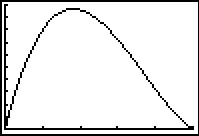
\includegraphics[width=2in]{./PolynomialsGraphics/Modeling01.jpg} \hspace{0.75in} & 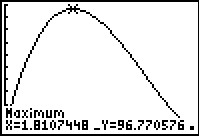
\includegraphics[width=2in]{./PolynomialsGraphics/Modeling02.jpg}

\end{tabular}
\end{center}
\vspace{-.55in} \qed
\end{enumerate}
\label{openbox}
\end{ex}


In order to solve Example \ref{openbox}, we made good use of the graph of the polynomial $y=V(x)$, so we ought to turn our attention to graphs of polynomials in general.  Below are the graphs of $y=x^2$, $y=x^4$ and $y=x^6$, side-by-side.  We have omitted the axes to allow you to see that as the exponent increases, the `bottom' becomes `flatter' and the `sides' become `steeper.'  If you take the the time to graph these functions by hand,\footnote{Make sure you choose some $x$-values between $-1$ and $1$.} you will see why. 

\smallskip

%\begin{tabular}{m{1in}m{1.5in}m{1.5in}m{1.5in}}

%&
\begin{center}
\begin{tabular}{ccc}

\begin{mfpic}[10][5]{-3.5}{3.5}{-1}{10}
\arrow \reverse \arrow \function{-3.1623,3.1623,0.1}{x**2}
\tcaption{$y=x^2$}
\end{mfpic}

\hspace{1in} &

\begin{mfpic}[10][5]{-2}{2}{-1}{10}
\arrow \reverse \arrow \function{-1.7783,1.7783,0.1}{x**4}
\tcaption{$y=x^4$}
\end{mfpic}

\hspace{1in} &

\begin{mfpic}[10][5]{-2}{2}{-1}{10}
\arrow \reverse \arrow \function{-1.4678,1.4678,0.1}{x**6}
\tcaption{$y=x^6$}
\end{mfpic}

\end{tabular}
\end{center}

All of these functions are even, (Do you remember how to show this?) and it is exactly because the exponent is even.\footnote{Herein lies one of the possible origins of the term `even' when applied to functions.} This symmetry is important, but we want to explore a different yet equally important feature of these functions which we can be seen graphically -- their \index{polynomial function ! end behavior}\index{end behavior ! of a function graph}\textbf{end behavior}.  

\smallskip

The end behavior of a function is a way to describe what is happening to the function values (the $y$-values) as the $x$-values approach the `ends' of the $x$-axis.\footnote{Of course, there are no ends to the $x$-axis.} That is, what happens to $y$ as $x$ becomes small without bound\footnote{We think of $x$ as becoming a very large (in the sense of its absolute value) \textit{negative} number far to the left of zero.} (written $x \rightarrow -\infty$) and, on the flip side, as $x$ becomes large without bound\footnote{We think of $x$ as moving far to the right of zero and becoming a very large \textit{positive} number.} (written $x \rightarrow \infty$).  

\smallskip

For example, given $f(x) = x^2$, as $x \rightarrow -\infty$, we imagine substituting $x=-100$, $x=-1000$, etc., into $f$ to get $f(-100)=10000$, $f(-1000)=1000000$, and so on. Thus  the function values are becoming larger and larger positive numbers (without bound).  To describe this behavior, we write: as $x \rightarrow -\infty$, $f(x) \rightarrow \infty$.  If we study the behavior of $f$ as $x \rightarrow \infty$, we see that in this case, too, $f(x) \rightarrow \infty$. (We told you that the symmetry was important!) The same can be said for any function of the form $f(x) = x^n$ where $n$ is an even natural number.   If we generalize just a bit to include vertical scalings and reflections across the $x$-axis,\footnote{See Theorems \ref{reflections} and \ref{vscalings} in Section \ref{Transformations}.} we have


\smallskip

\colorbox{ResultColor}{\bbm

\smallskip

\centerline{ \textbf{End Behavior of functions $f(x) = ax^{n}$, $n$ even.}}

\smallskip

Suppose $f(x) = a x^{n}$ where $a \neq 0$ is a real number and $n$ is an even natural number.  The end behavior of the graph of $y=f(x)$ matches one of the following: \index{end behavior ! of $f(x) = ax^{n}, n$ even}

\begin{itemize}

\item  for $a > 0$, as $x \rightarrow -\infty$, $f(x) \rightarrow \infty$ and as $x \rightarrow \infty$, $f(x) \rightarrow \infty$

\item  for $a < 0$, as $x \rightarrow -\infty$, $f(x) \rightarrow -\infty$ and as $x \rightarrow \infty$, $f(x) \rightarrow -\infty$

\end{itemize}

Graphically:

\begin{tabular}{m{1.5in}m{1.5in}m{1.5in}}

&

\begin{mfpic}[5]{-5}{5}{-1}{5}
\arrow \reverse \function{-5,-3, 0.1}{(x**2)/5}
\dotted \function{-3,3, 0.1}{(x**2)/5}
\arrow \function{3,5, 0.1}{(x**2)/5}
\tcaption{$a>0$}
\end{mfpic}

&

\begin{mfpic}[5]{-5}{5}{-5}{1}
\arrow \reverse \function{-5,-3, 0.1}{(0-(x**2))/5} 
\dotted \function{-3,3, 0.1}{-(x**2)/5}
\arrow \function{3,5, 0.1}{(0-(x**2))/5} 
\tcaption{$a<0$}
\end{mfpic} 

\end{tabular}

\vspace{-.2in}

\ebm}

\smallskip

We now turn our attention to functions of the form $f(x) = x^{n}$ where $n \geq 3$ is an odd natural number. (We ignore the case when $n=1$, since the graph of $f(x)=x$ is a line and doesn't fit the general pattern of higher-degree odd polynomials.) Below we have graphed $y=x^3$, $y=x^5$, and $y=x^7$.    The `flattening' and `steepening' that we saw with the even powers presents itself here as well, and, it should come as no surprise that all of these functions are odd.\footnote{And are, perhaps, the inspiration for the moniker `odd function'.}  The end behavior of these functions is all the same, with $f(x) \rightarrow -\infty$ as $x \rightarrow -\infty$ and $f(x) \rightarrow \infty$ as $x \rightarrow \infty$.


%\begin{tabular}{m{1in}m{1.5in}m{1.5in}m{1.5in}}


%&
\begin{center}

\begin{tabular}{ccc}

\begin{mfpic}[10][5]{-2}{2}{-5}{5}
\arrow \reverse \arrow \function{-1.700,1.700,0.1}{x**3}
\tcaption{$y=x^3$}
\end{mfpic}

\hspace{1in} &

\begin{mfpic}[10][5]{-2}{2}{-5}{5}
\arrow \reverse \arrow \function{-1.3800,1.3800,0.1}{x**5}
\tcaption{$y=x^5$}
\end{mfpic}

\hspace{1in} &

\begin{mfpic}[10][5]{-2}{2}{-5}{5}
\arrow \reverse \arrow \function{-1.2585,1.2585,0.1}{x**7}
\tcaption{$y=x^7$}
\end{mfpic}

\end{tabular}
\end{center}

As with the even degreed functions we studied earlier, we can generalize their end behavior.

\smallskip

\colorbox{ResultColor}{\bbm

\smallskip

\centerline{ \textbf{End Behavior of functions $f(x) = ax^{n}$, $n$ odd.}}

\smallskip

Suppose $f(x) = a x^{n}$ where $a \neq 0$ is a real number and $n \geq 3$ is an odd natural number.  The end behavior of the graph of $y=f(x)$ matches one of the following: \index{end behavior ! of $f(x) = ax^{n}, n$ odd}

\begin{itemize}

\item  for $a > 0$, as $x \rightarrow -\infty$, $f(x) \rightarrow -\infty$ and as $x \rightarrow \infty$, $f(x) \rightarrow \infty$

\item  for $a < 0$, as $x \rightarrow -\infty$, $f(x) \rightarrow \infty$ and as $x \rightarrow \infty$, $f(x) \rightarrow -\infty$

\end{itemize}

Graphically:

\medskip

\begin{tabular}{m{1.5in}m{1.5in}m{1.5in}}

&

\begin{mfpic}[5]{-5}{5}{-1}{5}
\arrow \reverse \function{-5,-3, 0.1}{0 - (x**2)/5}
\dotted \function{-3,0, 0.1}{-(x**2)/5}
\dotted \function{0,3, 0.1}{(x**2)/5}
\arrow \function{3,5, 0.1}{(x**2)/5}
\tcaption{$a>0$}
\end{mfpic}

&

\begin{mfpic}[5]{-5}{5}{-1}{5}
\arrow \reverse \function{-5,-3, 0.1}{(x**2)/5}
\dotted \function{-3,0, 0.1}{(x**2)/5}
\dotted \function{0,3, 0.1}{-(x**2)/5}
\arrow \function{3,5, 0.1}{0 - (x**2)/5}
\tcaption{$a<0$}
\end{mfpic}

\end{tabular}

\vspace{-.2in}

\ebm}

\smallskip

Despite having different end behavior, all functions of the form $f(x) = ax^{n}$ for natural numbers $n$ share two properties which help distinguish them from other animals in the algebra zoo:  they  are \index{continuous}\index{function ! continuous}\textbf{continuous} and \index{smooth}\index{function ! smooth}\textbf{smooth}.  While these concepts are formally defined using Calculus,\footnote{In fact, if you take Calculus, you'll find that smooth functions are automatically continuous, so that saying `polynomials are continuous and smooth' is redundant.} informally, graphs of continuous functions have no `breaks' or `holes' in them, and the graphs of smooth functions have no `sharp turns'.  It turns out that these traits are preserved when functions are added together, so general polynomial functions inherit these qualities.  Below we find the graph of a function which is neither smooth nor continuous, and to its right we have a graph of a polynomial, for comparison.  The function whose graph appears on the left fails to be continuous where it has a `break' or `hole' in the graph;  everywhere else, the function is continuous.  The function is continuous at the `corner' and the `cusp', but we consider these `sharp turns', so these are places where the function fails to be smooth.  Apart from these four places, the function is smooth and continuous.  Polynomial functions are smooth and continuous everywhere, as exhibited in the graph on the right.

\phantomsection
\label{cusppicture} 

\medskip

\begin{center}

%\begin{tabular}{m{0.25in}m{2.5in}m{2.5in}}

%& 

\begin{tabular}{cc}

\begin{mfpic}[15]{-5}{5}{-2}{5}
\arrow \polyline{(-3,2),(-5,4)}
\arrow \function{-3,-1.5,0.1}{1-(2/(x+1))}
\dashed \polyline{(-1,0),(-1,5)}
\arrow \parafcn{-1,1.75,0.1}{(t**3,(t**2)+1)} 
\point[3pt]{(-1,2)}
\gclear \circle{(3.375,3.25),0.1}
\circle{(3.375,3.25),0.1}
\tlabel[cc](-3,1.5){\tiny `corner'}
\tlabel[cc](-1,-0.5){\tiny`break'}
\tlabel[cc](0,0.5){\tiny`cusp'}
\tlabel[cc](3.375,2.5){\tiny`hole'}
\tcaption{\tiny  Pathologies not found on graphs of polynomials}
\end{mfpic}

\hspace{0.75in} &

\begin{mfpic}[15][7.5]{-5}{5}{-10}{10}
\arrow \reverse \arrow \function{-3,3.5,0.1}{0.5*x*(x+2)*(x-3)}
\tcaption{\tiny  The graph of a polynomial}
\end{mfpic}

\end{tabular}

\end{center}

The notion of smoothness is what tells us graphically that, for example, $f(x) = |x|$, whose graph is the characteristic `$\vee$' shape, cannot be a polynomial.  The notion of continuity is what allowed us to construct the sign diagram for quadratic inequalities as we did in Section \ref{Inequalities}.  This last result is formalized in the following theorem.
  
\smallskip

\colorbox{ResultColor}{\bbm

\begin{thm} \textbf{The Intermediate Value Theorem (Zero Version):}  Suppose $f$ is a continuous function on an interval containing $x=a$ and $x=b$ with $a<b$. If $f(a)$ and $f(b)$ have different signs, then $f$ has at least one zero between $x = a$ and $x = b$;  that is, for at least one real number $c$ such that $a < c < b$, we have $f(c) = 0$. \index{Intermediate Value Theorem ! polynomial zero version}


\label{IVT}
\end{thm}

\ebm}

\smallskip

The Intermediate Value Theorem is extremely profound;  it gets to the heart of what it means to be a real number, and is one of the most often used and under appreciated theorems in Mathematics.  With that being said, most students see the result as common sense since it says, geometrically, that the graph of a polynomial function cannot be above the $x$-axis at one point and below the $x$-axis at another point without crossing the $x$-axis somewhere in between.  The following example uses the Intermediate Value Theorem to establish a fact that that most students take for granted.  Many students, and sadly some instructors, will find it silly.

\begin{ex}  Use the Intermediate Value Theorem to establish that $\sqrt{2}$ is a real number.

\smallskip

{\bf Solution.}  Consider the polynomial function $f(x) = x^2 - 2$.  Then $f(1) = -1$ and $f(3) = 7$.  Since $f(1)$ and $f(3)$ have different signs, the Intermediate Value Theorem guarantees us a real number $c$ between $1$ and $3$ with $f(c) = 0$.  If $c^2 - 2 = 0$ then $c = \pm \sqrt{2}$.  Since $c$ is between $1$ and $3$, $c$ is positive, so $c = \sqrt{2}$. \qed

\end{ex}

Our primary use of the Intermediate Value Theorem is in the construction of sign diagrams, as in Section \ref{Inequalities}, since it guarantees us that polynomial functions are always positive $(+)$ or always negative $(-)$ on intervals which do not contain any of its zeros.  The general algorithm for polynomials is given below.

\smallskip
\colorbox{ResultColor}{\bbm

\centerline{\textbf{Steps for Constructing a Sign Diagram for a Polynomial Function}}

\smallskip

\hspace{.17in} Suppose $f$ is a polynomial function. \index{sign diagram ! polynomial function}

\begin{enumerate}

\item  Find the zeros of $f$ and place them on the number line with the number $0$ above them.

\item  Choose a real number, called a \textbf{test value}, in each of the intervals determined in step 1. 

\item  Determine the sign of $f(x)$ for each test value in step 2, and write that sign above the corresponding interval.

\end{enumerate}

\ebm}
\smallskip 

\begin{ex}  Construct a sign diagram for $f(x) = x^3 (x-3)^2 (x+2) \left(x^2+1\right)$.   Use it to give a rough sketch of the graph of  $y=f(x)$.  \label{polygraphex}

\smallskip

{\bf Solution.}  First, we find the zeros of $f$ by solving $x^3 (x-3)^2 (x+2)\left(x^2+1\right)=0$.   We get $x=0$, $x=3$ and $x=-2$. (The equation $x^2+1=0$ produces no real solutions.)  These three points divide the real number line into four intervals:  $(-\infty, -2)$, $(-2,0)$, $(0,3)$ and $(3,\infty)$.  We select the test values $x=-3$, $x=-1$, $x=1$ and $x=4$. We find $f(-3)$ is $(+)$, $f(-1)$ is $(-)$ and $f(1)$ is $(+)$ as is $f(4)$.  Wherever $f$ is $(+)$, its graph is above the $x$-axis;  wherever $f$ is $(-)$, its graph is below the $x$-axis.  The $x$-intercepts of the graph of $f$ are $(-2,0)$, $(0,0)$ and $(3,0)$.  Knowing $f$ is smooth and continuous allows us to sketch its graph.

\begin{tabular}{m{0.5in}m{2.5in}m{2.5in}}

&

\begin{mfpic}[10]{-8}{8}{-2}{30}
\arrow \reverse \arrow \polyline{(-8,0),(8,0)}
\xmarks{-3,0,3}
\arrow \polyline{(-5,-1.5),(-5,-0.5)}
\arrow \polyline{(-1.5,-1.5),(-1.5,-0.5)}
\arrow \polyline{(1.5,-1.5),(1.5,-0.5)}
\arrow \polyline{(5,-1.5),(5,-0.5)}
\tlpointsep{4pt}
\axislabels {x}{{$-2$} -3, {$0$} 0, {$3$} 3 }
\tlabel[cc](-5,1){$(+)$}
\tlabel[cc](-5,-2.25){$-3$}
\tlabel[cc](-3,1){$0$}
\tlabel[cc](-1.5,1){$(-)$}
\tlabel[cc](-1.75,-2.25){$-1$}
\tlabel[cc](0,1){$0$}
\tlabel[cc](1.5,1){$(+)$}
\tlabel[cc](1.5,-2.25){$1$}
\tlabel[cc](3,1){$0$}
\tlabel[cc](5,1){$(+)$}
\tlabel[cc](5,-2.25){$4$}
\end{mfpic} 

&

\begin{mfpic}[15]{-5}{5}{-2}{3}
\arrow \reverse \arrow \function{-2.2,3.5, 0.1}{0.05*((x)**3)*(x+2)*((x-3)**2)} 
\axes
\tlabel[cc](5,-0.5){\scriptsize $x$}
\tlabel[cc](0.5,3){\scriptsize $y$}
\point[3pt]{(-2,0), (0,0), (3,0)}
\xmarks{-4,-3,-2,-1,1,2,3,4}
\tcaption{ \scriptsize A sketch of $y=f(x)$}
\end{mfpic} 

\end{tabular}

\vspace{-.35in}

\qed

\end{ex}

A couple of notes about the Example \ref{polygraphex} are in order.  First, note that we purposefully did not label the $y$-axis in the sketch of the graph of $y=f(x)$.  This is because the sign diagram gives us the zeros and the relative position of the graph - it doesn't give us any information as to how high or low the graph strays from the $x$-axis.  Furthermore, as we have mentioned earlier in the text, without Calculus, the values of the relative maximum and minimum can only be found approximately using a calculator.  If we took the time to find the leading term of $f$, we would find it to be $x^8$.  Looking at the end behavior of $f$, we notice that it matches the end behavior of $y=x^8$.  This is no accident, as we find out in the next theorem.

\medskip

\colorbox{ResultColor}{\bbm

\begin{thm} \label{EBPolynomials}\index{end behavior ! polynomial}\textbf{End Behavior for Polynomial Functions:} The end behavior of a polynomial $f(x) = a_{n} x^{n} + a_{n-\mbox{\tiny$1$}} x^{n-\mbox{\tiny$1$}} + \ldots + a_{\mbox{\tiny $2$}} x^{\mbox{\tiny $2$}} + a_{\mbox{\tiny $1$}} x + a_{\mbox{\tiny $0$}}$ with $a_{n} \neq 0$ matches the end behavior of $y = a_{n} x^{n}$.  
\end{thm}

\ebm}

\medskip

To see why Theorem \ref{EBPolynomials} is true, let's first look at a specific example.  Consider $f(x) = 4x^3 - x + 5$.  If we wish to examine end behavior, we look to see the behavior of $f$ as $x \rightarrow \pm \infty$.  Since we're concerned with $x$'s far down the $x$-axis, we are far away from $x=0$ so can rewrite $f(x)$ for these values of $x$ as \[ f(x) = 4x^3 \left( 1 - \dfrac{1}{4x^2} + \dfrac{5}{4x^3}\right)\]

As $x$ becomes unbounded (in either direction), the terms $\frac{1}{4x^2}$ and $\frac{5}{4x^3}$ become closer and closer to $0$, as the table below indicates.


\[ \begin{array}{|r||r|r|}  

\hline 

 x & \frac{1}{4x^2} & \frac{5}{4x^3} \vphantom{\dfrac{a}{a}} \\ [2pt] \hline
-1000  & 0.00000025 & -0.00000000125 \\  \hline
-100  & 0.000025 & -0.00000125 \\  \hline
-10 & 0.0025 & -0.00125 \\  \hline
10  & 0.0025 & 0.00125 \\  \hline
100 & 0.000025 & 0.00000125 \\  \hline
1000 & 0.00000025 & 0.00000000125 \\  \hline
\end{array} \]

\smallskip

In other words, as $x \rightarrow \pm \infty$, $f(x) \approx 4x^3\left( 1 - 0 +0\right) = 4x^3$, which is the leading term of $f$.  The formal proof of Theorem \ref{EBPolynomials} works in much the same way.  Factoring out the leading term leaves

\[ f(x) = a_{n} x^{n} \left( 1 + \dfrac{a_{n-\mbox{\tiny$1$}}}{a_{n} x}+ \ldots + \dfrac{a_{\mbox{\tiny$2$}}}{a_{n} x^{n-2}} + \dfrac{a_{\mbox{\tiny$1$}}}{a_{n} x^{n-1}}+\dfrac{a_{\mbox{\tiny$0$}}}{a_{n} x^{n}}\right)\]

As $x \rightarrow \pm \infty$, any term with an $x$ in the denominator becomes closer and closer to $0$, and we have $f(x) \approx a_{n} x^{n}$.  Geometrically, Theorem \ref{EBPolynomials} says that if we graph $y=f(x)$ using a graphing calculator, and continue to `zoom out', the graph of it and its leading term become indistinguishable.  Below are the graphs of $y=4x^3-x+5$ (the thicker line) and $y=4x^3$ (the thinner line) in two different windows.

\begin{center}

\begin{tabular}{cc}

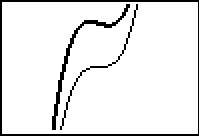
\includegraphics[width=2in]{./PolynomialsGraphics/EB01.jpg} \hspace{.25in} & 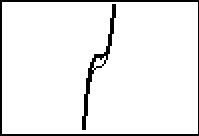
\includegraphics[width=2in]{./PolynomialsGraphics/EB02.jpg} \\

A view `close' to the origin. \hspace{.25in} & A `zoomed out' view. \\

\end{tabular}

\end{center}

Let's return to the function in Example \ref{polygraphex}, $f(x) = x^3 (x-3)^2 (x+2)\left(x^2+1\right)$, whose sign diagram and graph are reproduced below for reference.  Theorem \ref{EBPolynomials} tells us that the end behavior is the same as that of its leading term $x^{8}$.  This tells us that the graph of $y=f(x)$ starts and ends above the $x$-axis.  In other words, $f(x)$ is $(+)$ as $x \rightarrow \pm \infty$, and as a result, we no longer need to evaluate $f$ at the test values $x=-3$ and $x=4$.  Is there a way to eliminate the need to evaluate $f$ at the other test values?  What we would really need to know is how the function behaves near its zeros - does it cross through the $x$-axis at these points, as it does at $x=-2$ and $x=0$, or does it simply touch and rebound like it does at $x=3$.  From the sign diagram, the graph of $f$ will cross the $x$-axis whenever the signs on either side of the zero switch (like they do at $x=-2$ and $x=0$);  it will touch when the signs are the same on either side of the zero (as is the case with $x=3$). What we need to determine is the reason behind whether or not the sign change occurs.

\begin{tabular}{m{0.5in}m{2.5in}m{2.5in}}

&

\begin{mfpic}[10]{-8}{8}{-2}{2}
\arrow \reverse \arrow \polyline{(-8,0),(8,0)}
\xmarks{-3,0,3}
\arrow \polyline{(-5,-1.5),(-5,-0.5)}
\arrow \polyline{(-1.5,-1.5),(-1.5,-0.5)}
\arrow \polyline{(1.5,-1.5),(1.5,-0.5)}
\arrow \polyline{(5,-1.5),(5,-0.5)}
\tlpointsep{4pt}
\axislabels {x}{{$-2$} -3, {$0$} 0, {$3$} 3 }
\tlabel[cc](-5,1){$(+)$}
\tlabel[cc](-5,-2.25){$-3$}
\tlabel[cc](-3,1){$0$}
\tlabel[cc](-1.5,1){$(-)$}
\tlabel[cc](-1.75,-2.25){$-1$}
\tlabel[cc](0,1){$0$}
\tlabel[cc](1.5,1){$(+)$}
\tlabel[cc](1.5,-2.25){$1$}
\tlabel[cc](3,1){$0$}
\tlabel[cc](5,1){$(+)$}
\tlabel[cc](5,-2.25){$4$}
\end{mfpic} 

&

\begin{mfpic}[15]{-5}{5}{-2}{3}
\arrow \reverse \arrow \function{-2.2,3.5, 0.1}{0.05*((x)**3)*(x+2)*((x-3)**2)} 
\axes
\tlabel[cc](5,-0.5){\scriptsize $x$}
\tlabel[cc](0.5,3){\scriptsize $y$}
\point[3pt]{(-2,0), (0,0), (3,0)}
\xmarks{-4,-3,-2,-1,1,2,3,4}
\tcaption{ \scriptsize A sketch of $y=f(x)$}
\end{mfpic} 

\end{tabular}

Fortunately, $f$ was given to us in factored form:  $f(x) = x^3 (x-3)^2 (x+2)$.  When we attempt to determine the sign of $f(-4)$, we are attempting to find the sign of the number $(-4)^3 (-7)^2 (-2)$, which works out to be $(-)(+)(-)$ which is $(+)$.  If we move to the other side of $x=-2$, and find the sign of $f(-1)$, we are determining the sign of  $(-1)^3 (-4)^2 (+1)$, which is $(-)(+)(+)$ which gives us the $(-)$.  Notice that signs of the first two factors in both expressions are the same in $f(-4)$ and $f(-1)$.  The only factor which switches sign is the third factor, $(x+2)$, precisely the factor which gave us the zero $x=-2$.  If we move to the other side of $0$ and look closely at $f(1)$, we get the sign pattern $(+1)^3(-2)^2(+3)$ or $(+)(+)(+)$ and we note that, once again, going from $f(-1)$ to $f(1)$, the only factor which changed sign was the first factor, $x^3$, which corresponds to the zero $x=0$.  Finally, to find $f(4)$, we substitute to get $(+4)^3(+2)^2(+5)$ which is $(+)(+)(+)$ or $(+)$.  The sign didn't change for the middle factor $(x-3)^2$.  Even though this is the factor which corresponds to the zero $x=3$, the fact that the quantity is \textit{squared} kept the sign of the middle factor the same on either side of $3$.  If we look back at the exponents on the factors $(x+2)$ and $x^3$, we see that they are both odd, so as we substitute values to the left and right of the corresponding zeros, the signs of the corresponding factors change which results in the sign of the function value changing.  This is the key to the behavior of the function near the zeros.  We need a definition and then a theorem.

\smallskip

\colorbox{ResultColor}{\bbm

\begin{defn} \label{multiplicity} Suppose $f$ is a polynomial function and $m$ is a natural number. If $(x-c)^{m}$ is a factor of $f(x)$ but $(x-c)^{m+1}$ is not, then we say $x=c$ is a zero of \index{polynomial function ! zero ! multiplicity}\index{multiplicity ! of a zero}\index{zero ! multiplicity of}\textbf{multiplicity} $m$.

\end{defn}

\ebm}

\smallskip

Hence,  rewriting  $f(x) = x^3 (x-3)^2 (x+2)$ as $f(x) = (x-0)^3 (x-3)^2 (x-(-2))^{1}$, we see that $x=0$ is a zero of multiplicity $3$, $x=3$ is a zero of multiplicity $2$ and $x=-2$ is a zero of multiplicity $1$.

\smallskip

\colorbox{ResultColor}{\bbm

\begin{thm} \label{roleofmultiplicity} \textbf{The Role of Multiplicity:}  Suppose $f$ is a polynomial function  and $x=c$ is a zero of multiplicity $m$.  \index{multiplicity ! effect on the graph of a polynomial}

\begin{itemize}

\item  If $m$ is even, the graph of $y=f(x)$ touches and rebounds from the $x$-axis at $(c,0)$.

\item  If $m$ is odd, the graph of $y=f(x)$ crosses through the $x$-axis at $(c,0)$.

\end{itemize}

\end{thm}

\ebm}

\medskip

Our last example shows how end behavior and multiplicity allow us to sketch a decent graph without appealing to a sign diagram.

\begin{ex}  Sketch the graph of $f(x) = -3(2x-1)(x+1)^2$ using end behavior and the multiplicity of its zeros.

\bigskip

{ \bf Solution.}  The end behavior of the graph of $f$ will match that of its leading term.  To find the leading term, we multiply by the leading terms of each factor to get $(-3)(2x)(x)^2 = -6x^3$.  This tells us that the graph will start above the $x$-axis, in Quadrant II, and finish below the $x$-axis, in Quadrant IV.  Next, we find the zeros of $f$.  Fortunately for us, $f$ is factored.\footnote{Obtaining the factored form of a polynomial is the main focus of the next few sections.}  Setting each factor equal to zero gives is $x = \frac{1}{2}$ and $x=-1$ as zeros. To find the multiplicity of $x=\frac{1}{2}$ we note that it corresponds to the factor $(2x-1)$.  This isn't strictly in the form required in Definition \ref{multiplicity}.  If we factor out the $2$, however, we get $(2x-1) = 2\left(x-\frac{1}{2}\right)$, and we see that the multiplicity of $x = \frac{1}{2}$ is $1$.  Since $1$ is an odd number, we know from Theorem \ref{roleofmultiplicity} that the graph of $f$ will cross through the $x$-axis at $\left(\frac{1}{2},0\right)$.   Since the zero $x=-1$ corresponds to the factor $(x+1)^2 = (x-(-1))^2$, we find its multiplicity to be $2$ which is an even number.  As such, the graph of $f$ will touch and rebound from the $x$-axis at $(-1,0)$.  Though we're not asked to, we can find the $y$-intercept by finding $f(0) = -3(2(0)-1)(0+1)^2 = 3$.  Thus  $(0,3)$ is an additional point on the graph.  Putting this together gives us the graph below.

\begin{center}

\begin{mfpic}[20][10]{-3}{3}{-5}{5}
\arrow \reverse \arrow \function{-1.75,0.75,0.1}{0-1.5*(2*x-1)*((x+1)**2)}
\axes
\tlabel[cc](3,-0.5){\scriptsize $x$}
\tlabel[cc](0.5,5){\scriptsize $y$}
\point[3pt]{(0.5,0), (-1,0), (0,1.5) }
\xmarks{-2,-1,0,1,2}
\ymarks{0.5, 1.0, 1.5, 2}
\end{mfpic}

\end{center} 

\vspace{-.25in}

\qed

\end{ex}

\newpage

\subsection{Exercises}

In Exercises \ref{polyfactsfirst} - \ref{polyfactslast}, find the degree, the leading term, the leading coefficient, the constant term and the end behavior of the given polynomial.

\begin{multicols}{2}
\begin{enumerate}

\item  $f(x) = 4-x-3x^2$ \label{polyfactsfirst}
\item  $g(x) = 3x^5 - 2x^2 + x + 1$

\setcounter{HW}{\value{enumi}}
\end{enumerate}
\end{multicols}

\begin{multicols}{2}
\begin{enumerate}
\setcounter{enumi}{\value{HW}}

\item $q(r) = 1 - 16r^{4}$
\item $Z(b) = 42b - b^{3}$

\setcounter{HW}{\value{enumi}}
\end{enumerate}
\end{multicols}

\begin{multicols}{2}
\begin{enumerate}
\setcounter{enumi}{\value{HW}}

\item $f(x) = \sqrt{3}x^{17} + 22.5x^{10} - \pi x^{7} + \frac{1}{3}$
\item $s(t) = -4.9t^{2} + v_{\mbox{\tiny $0$}}t + s_{\mbox{\tiny $0$}}$

\setcounter{HW}{\value{enumi}}
\end{enumerate}
\end{multicols}

\begin{multicols}{2}
\begin{enumerate}
\setcounter{enumi}{\value{HW}}

\item $P(x) = (x - 1)(x - 2)(x - 3)(x - 4)$
\item $p(t) = -t^2(3 - 5t)(t^{2} + t + 4)$

\setcounter{HW}{\value{enumi}}
\end{enumerate}
\end{multicols}

\begin{multicols}{2}
\begin{enumerate}
\setcounter{enumi}{\value{HW}}

\item $f(x) = -2x^3(x+1)(x+2)^2$
\item $G(t) = 4(t-2)^2\left(t+\frac{1}{2}\right)$ \label{polyfactslast}

\setcounter{HW}{\value{enumi}}
\end{enumerate}
\end{multicols}

\phantomsection
\label{polygraphexercise}

In Exercises \ref{zeromultgraphfirst} - \ref{zeromultgraphlast}, find the real zeros of the given polynomial and their corresponding multiplicities.  Use this information along with a sign chart to provide a rough sketch of the graph of the polynomial.  Compare your answer with the result from a graphing utility.

\begin{multicols}{2}
\begin{enumerate}
\setcounter{enumi}{\value{HW}}

\item $a(x) = x(x + 2)^{2}$ \label{zeromultgraphfirst}
\item $g(x) = x(x + 2)^{3}$

\setcounter{HW}{\value{enumi}}
\end{enumerate}
\end{multicols}


\begin{multicols}{2}
\begin{enumerate}
\setcounter{enumi}{\value{HW}}

\item $f(x) = -2(x-2)^2(x+1)$
\item $g(x) = (2x+1)^2(x-3)$

\setcounter{HW}{\value{enumi}}
\end{enumerate}
\end{multicols}


\begin{multicols}{2}
\begin{enumerate}
\setcounter{enumi}{\value{HW}}

\item $F(x) = x^{3}(x + 2)^{2}$
\item $P(x) = (x - 1)(x - 2)(x - 3)(x - 4)$

\setcounter{HW}{\value{enumi}}
\end{enumerate}
\end{multicols}


\begin{multicols}{2}
\begin{enumerate}
\setcounter{enumi}{\value{HW}}

\item $Q(x) = (x + 5)^{2}(x - 3)^{4}$
\item $h(x) = x^2(x-2)^2(x+2)^2$

\setcounter{HW}{\value{enumi}}
\end{enumerate}
\end{multicols}


\begin{multicols}{2}
\begin{enumerate}
\setcounter{enumi}{\value{HW}}

\item $H(t) = (3-t)(t^2+1)$
\item $Z(b) = b(42 - b^{2})$ \label{zeromultgraphlast}

\setcounter{HW}{\value{enumi}}
\end{enumerate}
\end{multicols}

In Exercises \ref{polytransfirst} - \ref{polytranslast}, given the pair of functions $f$ and $g$, sketch the graph of $y=g(x)$ by starting with the graph of $y = f(x)$ and using transformations.  Track at least three points of your choice through the transformations. State the domain and range of $g$.

\begin{multicols}{2}
\begin{enumerate}
\setcounter{enumi}{\value{HW}}

\item $f(x) = x^3$,  $g(x) = (x + 2)^{3} + 1$ \label{polytransfirst}
\item $f(x) = x^4$, $g(x) = (x + 2)^{4} + 1$

\setcounter{HW}{\value{enumi}}
\end{enumerate}
\end{multicols}

\begin{multicols}{2}
\begin{enumerate}
\setcounter{enumi}{\value{HW}}

\item $f(x) = x^4$, $g(x) = 2 - 3(x - 1)^{4}$
\item $f(x) = x^5$, $g(x) = -x^{5} - 3$

\setcounter{HW}{\value{enumi}}
\end{enumerate}
\end{multicols}

\begin{multicols}{2}
\begin{enumerate}
\setcounter{enumi}{\value{HW}}

\item $f(x) = x^5$, $g(x) = (x+1)^5+10$
\item $f(x) = x^6$, $g(x) = 8-x^6$ \label{polytranslast}

\setcounter{HW}{\value{enumi}}
\end{enumerate}
\end{multicols}

\begin{enumerate}
\setcounter{enumi}{\value{HW}}

\item Use the Intermediate Value Theorem to prove that $f(x) = x^{3} - 9x + 5$ has a real zero in each of the following intervals: $[-4, -3], [0, 1]$ and $[2, 3]$.

\item  Rework Example \ref{boxnotopex} assuming the box is to be made from an 8.5 inch by 11 inch sheet of paper. Using scissors and tape, construct the box.  Are you surprised?\footnote{Consider decorating the box and presenting it to your instructor. If done well enough, maybe your instructor will issue you some bonus points.  Or maybe not.}

\setcounter{HW}{\value{enumi}}
\end{enumerate}

\phantomsection
\label{LCDmaxprofit} 

In Exercises \ref{lcdmaxprofitexerfirst} - \ref{lcdmaxprofitexerlast}, suppose the revenue $R$, in \textit{thousands} of dollars, from producing and selling $x$ \textit{hundred} LCD TVs is given by $R(x) = -5x^3+35x^2+155x$ for $0 \leq x \leq 10.07$.

\begin{enumerate}
\setcounter{enumi}{\value{HW}}

\item  Use a graphing utility to graph $y = R(x)$ and determine the number of TVs which should be sold to maximize revenue.  What is the maximum revenue? \label{lcdmaxprofitexerfirst}

\item Assume that the cost, in \textit{thousands} of dollars, to produce $x$ \textit{hundred} LCD TVs is given by $C(x) = 200x + 25$ for $x \geq 0$. Find and simplify an expression for the profit function $P(x)$.  (Remember: Profit = Revenue - Cost.)

\item  Use a graphing utility to graph $y = P(x)$ and determine the number of TVs which should be sold to maximize profit.  What is the maximum  profit? \label{lcdmaxprofitexerlast}

\item \label{newportaboycost} While developing their newest game, Sasquatch Attack!, the makers of the PortaBoy (from Example \ref{PortaBoyCost}) revised their cost function and now use $C(x) = .03x^{3} - 4.5x^{2} + 225x + 250$, for $x \geq 0$. As before, $C(x)$ is the cost to make $x$ PortaBoy Game Systems.  Market research indicates that the demand function $p(x) = -1.5x + 250$ remains unchanged.  Use a graphing utility to find the production level $x$ that maximizes the \textit{profit} made by producing and selling $x$ PortaBoy game systems.

\setcounter{HW}{\value{enumi}}
\end{enumerate}

\begin{enumerate}
\setcounter{enumi}{\value{HW}}

\item According to US Postal regulations, a rectangular shipping box must satisfy the inequality ``Length + Girth $\leq$ 130 inches'' for Parcel Post and ``Length + Girth $\leq$ 108 inches'' for other services. Let's assume we have a closed rectangular box with a square face of side length $x$ as drawn below.  The length is the longest side and is clearly labeled.  The girth is the distance around the box in the other two dimensions so in our case it is the sum of the four sides of the square, $4x$.  

\begin{enumerate}

\item \label{girthbox1} Assuming that we'll be mailing a box via Parcel Post where Length + Girth $=$ 130 inches, express the length of the box in terms of $x$ and then express the volume $V$ of the box in terms of $x$.

\item \label{girthbox2} Find the dimensions of the box of maximum volume that can be shipped via Parcel Post.

\item Repeat parts \ref{girthbox1} and \ref{girthbox2} if the box is shipped using ``other services''.

\end{enumerate}

\begin{center}

\begin{mfpic}[8]{-6}{12}{-1}{17}
\polyline{(0,0),(-4,3)}
\polyline{(-4,3), (-4,8)}
\polyline{(-4,8),(0,5)}
\polyline{(0,5),(0,0)}
\polyline{(0,0),(12,9)}
\polyline{(0,5),(12,14)}
\polyline{(-4,8),(8,17)}
\polyline{(8,17),(12,14)}
\polyline{(12,14),(12,9)}
\arrow \reverse \arrow \polyline{(0,-0.5),(12,8.5)}
\tlabel[cc](8,4){\tiny length}
\arrow \reverse \arrow \polyline{(-4, 2.5), (-0.5,-0.125)}
\tlabel[cc](-3,0.5){\tiny $x$}
\arrow \reverse \arrow \polyline{(-4.5, 3), (-4.5,8)}
\tlabel[cc](-5,5){\tiny $x$}
\end{mfpic}

\end{center}

\setcounter{HW}{\value{enumi}}
\end{enumerate}

\begin{enumerate}
\setcounter{enumi}{\value{HW}}


\item We now revisit the data set from Exercise \ref{regsunlight} in Section \ref{Regression}.  In that exercise, you were given a chart of the number of hours of daylight they get on the $21^{\mbox{st}}$ of each month in Fairbanks, Alaska based on the 2009 sunrise and sunset data found on the  \href{http://aa.usno.navy.mil/data/docs/RS_OneYear.php}{\underline{U.S. Naval Observatory}} website.  We let $x = 1$ represent January 21, 2009, $x = 2$ represent February 21, 2009, and so on.  The chart is given again for reference.

\medskip

\small

\noindent \begin{tabular}{|l|r|r|r|r|r|r|r|r|r|r|r|r|} \hline
Month  & & & & & & & & & & & & \\
Number & 1 & 2 & 3 & 4 & 5 & 6 & 7 & 8 & 9 & 10 & 11 & 12\\ 
\hline 
Hours of  & & & & & & & & & & & & \\
Daylight & 5.8 & 9.3 & 12.4 & 15.9 & 19.4 & 21.8 & 19.4 & 15.6 & 12.4 & 9.1 & 5.6 & 3.3 \\ \hline
\end{tabular}

\normalsize

\medskip

\noindent Find cubic (third degree) and quartic (fourth degree) polynomials which model this data and comment on the goodness of fit for each.  What can we say about using either model to make predictions about the year 2020?  (Hint: Think about the end behavior of polynomials.)  Use the models to see how many hours of daylight they got on your birthday and then check the website to see how accurate the models are.  Knowing that Sasquatch are largely nocturnal, what days of the year according to your models are going to allow for at least 14 hours of darkness for field research on the elusive creatures? 

\item \label{circuitexercisepoly} An electric circuit is built with a variable resistor installed.  For each of the following resistance values (measured in kilo-ohms, $k \Omega$),  the corresponding power to the load (measured in milliwatts, $mW$) is given in the table below. \footnote{The authors wish to thank Don Anthan and Ken White of Lakeland Community College for devising this problem and generating the accompanying data set.}

\noindent \begin{tabular}{|l|r|r|r|r|r|r|} \hline
Resistance: ($k \Omega$) & 1.012 & 2.199 & 3.275 & 4.676 & 6.805 & 9.975 \\ \hline
Power: ($mW$) & 1.063 & 1.496 & 1.610 & 1.613 & 1.505 & 1.314 \\ \hline
\end{tabular}

\begin{enumerate}

\item Make a scatter diagram of the data using the Resistance as the independent variable and Power as the dependent variable.

\item Use your calculator to find quadratic (2nd degree), cubic (3rd degree) and quartic (4th degree) regression models for the data and judge the reasonableness of each.

\item For each of the models found above, find the predicted maximum power that can be delivered to the load.  What is the corresponding resistance value?

\item Discuss with your classmates the limitations of these models - in particular, discuss the end behavior of each.

\end{enumerate}

\item Show that the end behavior of a linear function $f(x) = mx + b$ is as it should be according to the results we've established in the section for polynomials of odd degree.\footnote{Remember, to be a linear function, $m \neq 0$.}  (That is, show that the graph of a linear function is ``up on one side and down on the other'' just like the graph of $y = a_{n}x^{n}$ for odd numbers $n$.)

\item \index{multiplicity ! effect on the graph of a polynomial} There is one subtlety about the role of multiplicity that we need to discuss further; specifically we need to see `how' the graph crosses the $x$-axis at a zero of odd multiplicity.  In the section, we deliberately excluded the function $f(x) = x$ from the discussion of the end behavior of $f(x) = x^{n}$ for odd numbers $n$ and we said at the time that it was due to the fact that $f(x) = x$ didn't fit the pattern we were trying to establish.  You just showed in the previous exercise that the end behavior of a linear function behaves like every other polynomial of odd degree, so what doesn't $f(x) = x$ do that $g(x) = x^{3}$ does?  It's the `flattening' for values of $x$ near zero.  It is this local behavior that will distinguish between a zero of multiplicity 1 and one of higher odd multiplicity.  Look again closely at the graphs of $a(x) = x(x + 2)^{2}$ and $F(x) = x^{3}(x + 2)^{2}$ from Exercise \ref{polygraphexercise}.  Discuss with your classmates how the graphs are fundamentally different at the origin.  It might help to use a graphing calculator to zoom in on the origin to see the different crossing behavior. Also compare the behavior of $a(x) = x(x + 2)^{2}$ to that of $g(x) = x(x + 2)^{3}$ near the point $(-2, 0)$.  What do you predict will happen at the zeros of $f(x) = (x - 1)(x - 2)^2(x - 3)^{3}(x - 4)^{4}(x - 5)^{5}$?

\item Here are a few other questions for you to discuss with your classmates.  

\begin{enumerate}

\item How many local extrema could a polynomial of degree $n$ have?  How few local extrema can it have?
\item Could a polynomial have two local maxima but no local minima?  
\item If a polynomial has two local maxima and two local minima, can it be of odd degree?  Can it be of even degree?
\item Can a polynomial have local extrema without having any real zeros?
\item Why must every polynomial of odd degree have at least one real zero?
\item Can a polynomial have two distinct real zeros and no local extrema?
\item Can an $x$-intercept yield a local extrema?  Can it yield an absolute extrema?
\item If the $y$-intercept yields an absolute minimum, what can we say about the degree of the polynomial and the sign of the leading coefficient?   

\end{enumerate}

\setcounter{HW}{\value{enumi}}
\end{enumerate}
\newpage

\subsection{Answers}

\begin{multicols}{2}
\begin{enumerate}

\item $f(x) = 4-x-3x^2$ \\
Degree 2 \\
Leading term $-3x^{2}$\\
Leading coefficient $-3$\\
Constant term $4$\\
As $x \rightarrow -\infty, \; f(x) \rightarrow -\infty$\\
As $x \rightarrow \infty, \; f(x) \rightarrow -\infty$\\

\item  $g(x) = 3x^5 - 2x^2 + x + 1$ \\
Degree 5 \\
Leading term $3x^5$\\
Leading coefficient $3$\\
Constant term $1$\\
As $x \rightarrow -\infty, \; g(x) \rightarrow -\infty$\\
As $x \rightarrow \infty, \; g(x) \rightarrow \infty$\\


\setcounter{HW}{\value{enumi}}
\end{enumerate}
\end{multicols}

\begin{multicols}{2}
\begin{enumerate}
\setcounter{enumi}{\value{HW}}

\item $q(r) = 1 - 16r^{4}$\\
Degree 4 \\
Leading term $-16r^{4}$\\
Leading coefficient $-16$\\
Constant term $1$\\
As $r \rightarrow -\infty, \; q(r) \rightarrow -\infty$\\
As $r \rightarrow \infty, \; q(r) \rightarrow -\infty$\\

\item $Z(b) = 42b - b^{3}$\\
Degree 3 \\
Leading term $-b^{3}$\\
Leading coefficient $-1$\\
Constant term $0$\\
As $b \rightarrow -\infty, \; Z(b) \rightarrow \infty$\\
As $b \rightarrow \infty, \; Z(b) \rightarrow -\infty$\\

\setcounter{HW}{\value{enumi}}
\end{enumerate}
\end{multicols}

\begin{multicols}{2}
\begin{enumerate}
\setcounter{enumi}{\value{HW}}

\item $f(x) = \sqrt{3}x^{17} + 22.5x^{10} - \pi x^{7} + \frac{1}{3}$\\
Degree 17 \\
Leading term $\sqrt{3}x^{17}$\\
Leading coefficient $\sqrt{3}$\\
Constant term $\frac{1}{3}$\\
As $x \rightarrow -\infty, \; f(x) \rightarrow -\infty$\\
As $x \rightarrow \infty, \; f(x) \rightarrow \infty$\\


\item $s(t) = -4.9t^{2} + v_{\mbox{\tiny $0$}}t + s_{\mbox{\tiny $0$}}$\\
Degree 2 \\
Leading term $-4.9t^{2}$\\
Leading coefficient $-4.9$\\
Constant term $s_{\mbox{\tiny $0$}}$\\
As $t \rightarrow -\infty, \; s(t) \rightarrow -\infty$\\
As $t \rightarrow \infty, \; s(t) \rightarrow -\infty$\\


\setcounter{HW}{\value{enumi}}
\end{enumerate}
\end{multicols}

\begin{multicols}{2}
\begin{enumerate}
\setcounter{enumi}{\value{HW}}


\item $P(x) = (x - 1)(x - 2)(x - 3)(x - 4)$\\
Degree 4 \\
Leading term $x^{4}$\\
Leading coefficient $1$\\
Constant term $24$\\
As $x \rightarrow -\infty, \; P(x) \rightarrow \infty$\\
As $x \rightarrow \infty, \; P(x) \rightarrow \infty$\\

\item $p(t) = -t^2(3 - 5t)(t^{2} + t + 4)$\\
Degree 5 \\
Leading term $5t^{5}$\\
Leading coefficient $5$\\
Constant term $0$\\
As $t \rightarrow -\infty, \; p(t) \rightarrow -\infty$\\
As $t \rightarrow \infty, \; p(t) \rightarrow \infty$\\

\setcounter{HW}{\value{enumi}}
\end{enumerate}
\end{multicols}

\pagebreak

\begin{multicols}{2}
\begin{enumerate}
\setcounter{enumi}{\value{HW}}

\item $f(x) = -2x^3(x+1)(x+2)^2$ \\
Degree 6 \\
Leading term $-2x^{6}$\\
Leading coefficient $-2$\\
Constant term $0$\\
As $x \rightarrow -\infty, \; f(x) \rightarrow -\infty$\\
As $x \rightarrow \infty, \; f(x) \rightarrow -\infty$\\

\item $G(t) = 4(t-2)^2\left(t+\frac{1}{2}\right)$ \\
Degree 3 \\
Leading term $4t^3$\\
Leading coefficient $4$\\
Constant term $8$\\
As $t \rightarrow -\infty, \; G(t) \rightarrow -\infty$\\
As $t \rightarrow \infty, \; G(t) \rightarrow \infty$\\

\setcounter{HW}{\value{enumi}}
\end{enumerate}
\end{multicols}

\begin{multicols}{2}
\begin{enumerate}
\setcounter{enumi}{\value{HW}}

\item $a(x) = x(x + 2)^{2}$\\
$x = 0$ multiplicity 1\\
$x = -2$ multiplicity 2\\

\begin{mfpic}[20][10]{-3}{1}{-3}{5}
\arrow \reverse \arrow \function{-3,0.65,0.1}{x*((x + 2)**2)}
\axes
\tlabel[cc](1,-0.5){\scriptsize $x$}
\tlabel[cc](0.25,5){\scriptsize $y$}
\point[3pt]{(-2,0), (0,0)}
\xmarks{-2,-1}
\tiny
\tlpointsep{4pt}
\axislabels {x}{{$-2 \hspace{6pt}$} -2, {$-1 \hspace{6pt}$} -1}
\normalsize
\end{mfpic}

\vfill

\columnbreak

\item $g(x) = x(x + 2)^{3}$\\
$x = 0$ multiplicity 1\\
$x = -2$ multiplicity 3\\

\begin{mfpic}[20][20]{-3}{1}{-2}{5}
\arrow \reverse \arrow \function{-3,0.3,0.1}{x*((x + 2)**3)}
\axes
\tlabel[cc](1,-0.5){\scriptsize $x$}
\tlabel[cc](0.25,5){\scriptsize $y$}
\point[3pt]{(-2,0), (0,0)}
\xmarks{-2,-1}
\tiny
\tlpointsep{4pt}
\axislabels {x}{{$-2 \hspace{6pt}$} -2, {$-1 \hspace{6pt}$} -1}
\normalsize
\end{mfpic}


\setcounter{HW}{\value{enumi}}
\end{enumerate}
\end{multicols}

\begin{multicols}{2}
\begin{enumerate}
\setcounter{enumi}{\value{HW}}

\item $f(x) = -2(x-2)^2(x+1)$\\
$x=2$ multiplicity 2 \\
$x=-1$ multiplicity 1\\

\begin{mfpic}[20][10]{-3}{3}{-4}{4}
\arrow \reverse \arrow \function{-1.70,3.45,0.1}{(-0.4)*((x-2)**2)*(x+1)}
\axes
\tlabel[cc](3,-0.5){\scriptsize $x$}
\tlabel[cc](0.25,4){\scriptsize $y$}
\point[3pt]{(2,0), (-1,0)}
\xmarks{-2,-1,1,2}
\tiny
\tlpointsep{4pt}
\axislabels {x}{{$-2 \hspace{6pt}$} -2, {$-1 \hspace{6pt}$} -1, {$1$} 1, {$2$} 2}
\normalsize
\end{mfpic}



\item $g(x) = (2x+1)^2(x-3)$\\
$x=-\frac{1}{2}$ multiplicity 2 \\
$x=3$ multiplicity 1\\

\begin{mfpic}[20][10]{-2}{4}{-4}{4}
\arrow \reverse \arrow \function{-1.5,3.3,0.1}{(0.5)*((x+0.5)**2)*(x-3)}
\axes
\tlabel[cc](4,-0.5){\scriptsize $x$}
\tlabel[cc](0.25,4){\scriptsize $y$}
\point[3pt]{(-0.5,0), (3,0)}
\xmarks{-1,1,2,3}
\tiny
\tlpointsep{4pt}
\axislabels {x}{{$-1 \hspace{6pt}$} -1, {$1$} 1, {$2$} 2, {$3$} 3}
\normalsize
\end{mfpic}



\setcounter{HW}{\value{enumi}}
\end{enumerate}
\end{multicols}

\pagebreak

\begin{multicols}{2}
\begin{enumerate}
\setcounter{enumi}{\value{HW}}

\item $F(x) = x^{3}(x + 2)^{2}$\\
$x = 0$ multiplicity 3\\
$x = -2$ multiplicity 2\\

\begin{mfpic}[20][10]{-3}{1}{-3}{5}
\arrow \reverse \arrow \function{-2.45,0.85,0.1}{(x**3)*((x + 2)**2)}
\axes
\tlabel[cc](1,-0.5){\scriptsize $x$}
\tlabel[cc](0.25,5){\scriptsize $y$}
\point[3pt]{(-2,0), (0,0)}
\xmarks{-2,-1}
\tiny
\tlpointsep{4pt}
\axislabels {x}{{$-2 \hspace{6pt}$} -2, {$-1 \hspace{6pt}$} -1}
\normalsize
\end{mfpic}

\vfill

\columnbreak

\item $P(x) = (x - 1)(x - 2)(x - 3)(x - 4)$\\
$x = 1$ multiplicity 1\\
$x = 2$ multiplicity 1\\
$x = 3$ multiplicity 1\\
$x = 4$ multiplicity 1\\

\begin{mfpic}[20][10]{0}{5}{-1}{5}
\arrow \reverse \arrow \function{0.6,4.4,0.1}{(x - 1)*(x - 2)*(x - 3)*(x - 4)}
\axes
\tlabel[cc](5,-0.5){\scriptsize $x$}
\tlabel[cc](0.25,5){\scriptsize $y$}
\point[3pt]{(1,0),(2,0),(3,0),(4,0)}
\xmarks{1,2,3,4}
\tiny
\tlpointsep{4pt}
\axislabels {x}{{$1$} 1, {$2$} 2, {$3$} 3, {$4$} 4}
\normalsize
\end{mfpic}

\setcounter{HW}{\value{enumi}}
\end{enumerate}
\end{multicols}


\begin{multicols}{2}
\begin{enumerate}
\setcounter{enumi}{\value{HW}}


\item $Q(x) = (x + 5)^{2}(x - 3)^{4}$\\
$x = -5$ multiplicity 2\\
$x = 3$ multiplicity 4\\

\begin{mfpic}[10][20]{-6}{6}{-1}{3}
\arrow \reverse \arrow \function{-5.9,5.6,0.1}{(((x + 5)**2)*((x - 3)**4))/2000}
\axes
\tlabel[cc](6,-0.5){\scriptsize $x$}
\tlabel[cc](0.5,3){\scriptsize $y$}
\point[3pt]{(-5,0),(3,0)}
\xmarks{-5 step 1 until 5}
\tiny
\tlpointsep{4pt}
\axislabels {x}{{$-5 \hspace{6pt}$} -5, {$-4 \hspace{6pt}$} -4, {$-3 \hspace{6pt}$} -3, {$-2 \hspace{6pt}$} -2, {$-1 \hspace{6pt}$} -1, {$1$} 1, {$2$} 2, {$3$} 3, {$4$} 4, {$5$} 5}
\normalsize
\end{mfpic}

\vfill

\columnbreak

\item $f(x) = x^2(x-2)^2(x+2)^2$\\
$x = -2$ multiplicity 2\\
$x = 0$ multiplicity 2\\
$x = 2$ multiplicity 2\\

\begin{mfpic}[20][10]{-3}{3}{-1}{5}
\arrow \reverse \arrow \function{-2.45,2.45,0.1}{(0.2)*(x**2)*((x-2)**2)*((x+2)**2)}
\axes
\tlabel[cc](3,-0.5){\scriptsize $x$}
\tlabel[cc](0.5,5){\scriptsize $y$}
\point[3pt]{(-2,0), (0,0), (2,0)}
\xmarks{-2 step 1 until 2}
\tiny
\tlpointsep{4pt}
\axislabels {x}{{$-2 \hspace{6pt}$} -2, {$-1 \hspace{6pt}$} -1, {$1$} 1, {$2$} 2}
\normalsize
\end{mfpic}

\setcounter{HW}{\value{enumi}}
\end{enumerate}
\end{multicols}

\begin{multicols}{2}
\begin{enumerate}
\setcounter{enumi}{\value{HW}}

\item $H(t) = (3-t)\left(t^2+1\right)$\\
$x =3$ multiplicity 1\\

\begin{mfpic}[20][10]{-1}{4}{-4}{4}
\arrow \reverse \arrow \function{-0.75,3.3,0.1}{(0.5)*(3-x)*((x**2)+1)}
\axes
\tlabel[cc](4,-0.5){\scriptsize $t$}
\tlabel[cc](0.5,3){\scriptsize $y$}
\point[3pt]{(3,0)}
\xmarks{1 step 1 until 3}
\tiny
\tlpointsep{4pt}
\axislabels {x}{{$1$} 1, {$2$} 2, {$3$} 3}
\normalsize
\end{mfpic}

\vfill

\columnbreak

\item $Z(b) = b(42 - b^{2})$\\
$b = -\sqrt{42}$ multiplicity 1\\
$b = 0$ multiplicity 1\\
$b = \sqrt{42}$ multiplicity 1\\

\begin{mfpic}[10]{-7}{7}{-6}{6}
\arrow \reverse \arrow \function{-7,7,0.1}{(42*x - x**3)/20}
\axes
\tlabel[cc](7,-0.5){\scriptsize $b$}
\tlabel[cc](0.5,6){\scriptsize $y$}
\point[3pt]{(-6.4807,0),(0,0),(6.4807,0)}
\xmarks{-6 step 1 until 6}
\tiny
\tlpointsep{4pt}
\axislabels {x}{{$-6 \hspace{6pt}$} -6, {$-5 \hspace{6pt}$} -5, {$-4 \hspace{6pt}$} -4, {$-3 \hspace{6pt}$} -3, {$-2 \hspace{6pt}$} -2, {$-1 \hspace{6pt}$} -1, {$1$} 1, {$2$} 2, {$3$} 3, {$4$} 4, {$5$} 5, {$6$} 6}
\normalsize
\end{mfpic}

\setcounter{HW}{\value{enumi}}
\end{enumerate}
\end{multicols}

\pagebreak

\begin{multicols}{2}
\begin{enumerate}
\setcounter{enumi}{\value{HW}}

\item $g(x) = (x + 2)^{3} + 1$ \\ 
domain: $(-\infty, \infty)$ \\ 
range: $(-\infty, \infty)$ \\

\begin{mfpic}[20][8]{-5}{1}{-11}{13}
\arrow \reverse \arrow \function{-4.25,0.25,0.1}{((x + 2)**3) + 1}
\axes
\tlabel[cc](1,-0.75){\scriptsize $x$}
\tlabel[cc](0.5,13){\scriptsize $y$}
\point[3pt]{(-4,-7),(-3,0),(-2,1),(-1,2),(0,9)}
\xmarks{-4,-3,-2,-1}
\ymarks{-10 step 1 until 12}
\tiny
\tlpointsep{4pt}
\axislabels {x}{{$-4 \hspace{6pt}$} -4, {$-3 \hspace{6pt}$} -3, {$-2 \hspace{6pt}$} -2, {$-1 \hspace{6pt}$} -1}
\axislabels {y}{{$-10$} -10, {$-9$} -9, {$-8$} -8, {$-7$} -7, {$-6$} -6, {$-5$} -5, {$-4$} -4, {$-3$} -3, {$-2$} -2, {$-1$} -1, {$1$} 1, {$2$} 2, {$3$} 3, {$4$} 4, {$5$} 5, {$6$} 6, {$7$} 7, {$8$} 8, {$9$} 9, {$10$} 10, {$11$} 11, {$12$} 12}
\normalsize
\end{mfpic}

\vfill

\columnbreak

\item $g(x) = (x + 2)^{4} + 1$\\
domain: $(-\infty, \infty)$\\
range: $[1, \infty)$\\

\begin{mfpic}[20][8]{-5}{1}{-1}{22}
\arrow \reverse \arrow \function{-4.12,0.12,0.1}{((x + 2)**4) + 1}
\axes
\tlabel[cc](1,-0.75){\scriptsize $x$}
\tlabel[cc](0.5,22){\scriptsize $y$}
\point[3pt]{(-4,17),(-3,2),(-2,1),(-1,2),(0,17)}
\xmarks{-4,-3,-2,-1}
\ymarks{1 step 1 until 21}
\tiny
\tlpointsep{4pt}
\axislabels {x}{{$-4 \hspace{6pt}$} -4, {$-3 \hspace{6pt}$} -3, {$-2 \hspace{6pt}$} -2, {$-1 \hspace{6pt}$} -1}
\axislabels {y}{{$1$} 1, {$2$} 2, {$3$} 3, {$4$} 4, {$5$} 5, {$6$} 6, {$7$} 7, {$8$} 8, {$9$} 9, {$10$} 10, {$11$} 11, {$12$} 12, {$13$} 13, {$14$} 14, {$15$} 15, {$16$} 16, {$17$} 17, {$18$} 18, {$19$} 19, {$20$} 20, {$21$} 21}
\normalsize
\end{mfpic}

\setcounter{HW}{\value{enumi}}
\end{enumerate}
\end{multicols}

\begin{multicols}{2}
\begin{enumerate}
\setcounter{enumi}{\value{HW}}


\item $g(x) = 2 - 3(x - 1)^{4}$\\
domain: $(-\infty, \infty)$\\
range: $(-\infty, 2]$\\

\begin{mfpic}[20][8]{-1}{3}{-14}{3}
\arrow \reverse \arrow \function{-0.5,2.5,0.1}{2 - 3*((x - 1)**4)}
\axes
\tlabel[cc](3,-0.75){\scriptsize $x$}
\tlabel[cc](0.5,3){\scriptsize $y$}
\point[3pt]{(1,2),(0,-1),(2,-1)}
\xmarks{1,2}
\ymarks{-13 step 1 until 2}
\tiny
\tlpointsep{4pt}
\axislabels {x}{{$1$} 1, {$2$} 2}
\axislabels {y}{{$-13$} -13, {$-12$} -12, {$-11$} -11, {$-10$} -10, {$-9$} -9, {$-8$} -8, {$-7$} -7, {$-6$} -6, {$-5$} -5, {$-4$} -4, {$-3$} -3, {$-2$} -2, {$-1$} -1, {$1$} 1, {$2$} 2}
\normalsize
\end{mfpic}


\vfill

\columnbreak

\item $g(x) = -x^{5} - 3$\\
domain: $(-\infty, \infty)$\\
range: $(-\infty, \infty)$\\

\begin{mfpic}[20][8]{-2}{2}{-11}{11}
\arrow \reverse \arrow \function{-1.68,1.5,0.1}{-(x**5) - 3}
\axes
\tlabel[cc](2,-0.75){\scriptsize $x$}
\tlabel[cc](0.5,11){\scriptsize $y$}
\point[3pt]{(-1,-2),(0,-3),(1,-4)}
\xmarks{-1,1}
\ymarks{-10 step 1 until 10}
\tiny
\tlpointsep{4pt}
\axislabels {x}{{$-1 \hspace{6pt}$} -1, {$1$} 1}
\axislabels {y}{{$-10$} -10, {$-9$} -9, {$-8$} -8, {$-7$} -7, {$-6$} -6, {$-5$} -5, {$-4$} -4, {$-3$} -3, {$-2$} -2, {$-1$} -1, {$1$} 1, {$2$} 2, {$3$} 3, {$4$} 4, {$5$} 5, {$6$} 6, {$7$} 7, {$8$} 8, {$9$} 9, {$10$} 10}
\normalsize
\end{mfpic}


\setcounter{HW}{\value{enumi}}
\end{enumerate}
\end{multicols}


\pagebreak

\begin{multicols}{2}
\begin{enumerate}

\setcounter{enumi}{\value{HW}}
\item $g(x) = (x+1)^5+10$\\
domain: $(-\infty, \infty)$\\
range: $(-\infty, \infty)$\\

\begin{mfpic}[20][8]{-5}{1}{-1}{22}
\arrow \reverse \arrow \function{-2.64,0.58,0.1}{((x + 1)**5) + 10}
\axes
\tlabel[cc](1,-0.75){\scriptsize $x$}
\tlabel[cc](0.5,22){\scriptsize $y$}
\point[3pt]{(0,11), (-1,10), (-2,9)}
\xmarks{-4,-3,-2,-1}
\ymarks{1 step 1 until 21}
\tiny
\tlpointsep{4pt}
\axislabels {x}{{$-4 \hspace{6pt}$} -4, {$-3 \hspace{6pt}$} -3, {$-2 \hspace{6pt}$} -2, {$-1 \hspace{6pt}$} -1}
\axislabels {y}{{$1$} 1, {$2$} 2, {$3$} 3, {$4$} 4, {$5$} 5, {$6$} 6, {$7$} 7, {$8$} 8, {$9$} 9, {$10$} 10, {$11$} 11, {$12$} 12, {$13$} 13, {$14$} 14, {$15$} 15, {$16$} 16, {$17$} 17, {$18$} 18, {$19$} 19, {$20$} 20, {$21$} 21}
\normalsize
\end{mfpic}


\vfill

\columnbreak

\item $g(x) = 8-x^{6}$\\
domain: $(-\infty, \infty)$\\
range: $(-\infty, 8]$\\

\begin{mfpic}[20][8]{-2}{2}{-11}{11}
\arrow \reverse \arrow \function{-1.6,1.6,0.1}{8-(x**6)}
\axes
\tlabel[cc](2,-0.75){\scriptsize $x$}
\tlabel[cc](0.5,11){\scriptsize $y$}
\point[3pt]{(-1,7),(0,8),(1,7)}
\xmarks{-1,1}
\ymarks{-10 step 1 until 10}
\tiny
\tlpointsep{4pt}
\axislabels {x}{{$-1 \hspace{6pt}$} -1, {$1$} 1}
\axislabels {y}{{$-10$} -10, {$-9$} -9, {$-8$} -8, {$-7$} -7, {$-6$} -6, {$-5$} -5, {$-4$} -4, {$-3$} -3, {$-2$} -2, {$-1$} -1, {$1$} 1, {$2$} 2, {$3$} 3, {$4$} 4, {$5$} 5, {$6$} 6, {$7$} 7, {$8$} 8, {$9$} 9, {$10$} 10}
\normalsize
\end{mfpic}


\setcounter{HW}{\value{enumi}}
\end{enumerate}
\end{multicols}

\begin{enumerate}
\setcounter{enumi}{\value{HW}}

\item We have $f(-4)=-23,\; f(-3)=5,\; f(0)=5,\; f(1)=-3,\; f(2)=-5\;$ and $f(3)=5$ so the Intermediate Value Theorem tells us that $f(x) = x^{3} - 9x + 5$ has real zeros in the intervals $[-4, -3], [0, 1]$ and $[2, 3]$.

\item  $V(x) = x(8.5-2x)(11-2x) = 4x^3-39x^2+93.5x$, $0 < x < 4.25$.  Volume is maximized when $x \approx 1.58$, so the dimensions of the box with maximum volume are: height $\approx$ 1.58 inches, width $\approx$ 5.34 inches, and depth $\approx$ 7.84 inches.  The maximum volume is $\approx$ 66.15 cubic inches.


\item The calculator gives the location  of the absolute maximum (rounded to three decimal places) as $x \approx 6.305$ and $y \approx 1115.417$.  Since $x$ represents the number of TVs sold in hundreds, $x = 6.305$ corresponds to $630.5$ TVs.  Since we can't sell half of a TV, we compare $R(6.30) \approx 1115.415$ and $R(6.31) \approx 1115.416$, so selling $631$ TVs results in a (slightly) higher revenue.  Since $y$ represents the revenue in \textit{thousands} of dollars, the maximum revenue is $\$ 1,\!115,\!416$.

\item $P(x) = R(x) - C(x) = -5x^3+35x^2-45x-25$, $0 \leq x \leq 10.07$.

\item  The calculator gives the location  of the absolute maximum (rounded to three decimal places) as $x \approx 3.897$ and $y \approx 35.255$.  Since $x$ represents the number of TVs sold in hundreds, $x = 3.897$ corresponds to $389.7$ TVs.  Since we can't sell $0.7$ of a TV, we compare $P(3.89) \approx 35.254$ and $P(3.90) \approx 35.255$, so selling $390$ TVs results in a (slightly) higher revenue.  Since $y$ represents the revenue in \textit{thousands} of dollars, the maximum revenue is $\$ 35,\!255$.

\item Making and selling 71 PortaBoys yields a maximized profit of \$5910.67.


\item \begin{enumerate}

\item Our ultimate goal is to maximize the volume, so we'll start with the maximum Length $+$ Girth of $130.$  This means the length is $130 - 4x$.  The volume of a rectangular box is always length $\times$ width $\times$ height so we get $V(x) = x^{2}(130 - 4x) = -4x^{3} + 130x^{2}$.  

\item Graphing $y = V(x)$ on $[0, 33] \times [0, 21000]$ shows a maximum at $(21.67, 20342.59)$ so the dimensions of the box with maximum volume are $21.67\mbox{in.} \times 21.67\mbox{in.} \times 43.32\mbox{in.}$ for a volume of $20342.59\mbox{in.}^{3}$.

\item If we start with Length $+$ Girth $= 108$ then the length is $108 - 4x$ and the volume is $V(x) = -4x^{3} + 108x^{2}$.  Graphing $y = V(x)$ on $[0, 27] \times [0, 11700]$ shows a maximum at $(18.00, 11664.00)$ so the dimensions of the box with maximum volume are $18.00\mbox{in.} \times 18.00\mbox{in.} \times 36\mbox{in.}$ for a volume of $11664.00\mbox{in.}^{3}$.  (Calculus will confirm that the measurements which maximize the volume are \underline{exactly} 18in. by 18in. by 36in., however, as I'm sure you are aware by now, we treat all calculator results as approximations and list them as such.)

\end{enumerate}

\setcounter{HW}{\value{enumi}}
\end{enumerate}




\begin{enumerate}
\setcounter{enumi}{\value{HW}}


\item The cubic regression model is $p_{\mbox{\tiny $3$}}(x) = 0.0226x^{3} - 0.9508x^{2} + 8.615x - 3.446$.  It has $R^{2} = 0.93765$ which isn't bad.  The graph of $y = p_{\mbox{\tiny $3$}}(x)$ in the viewing window $[-1,13] \times [0, 24]$ along with the scatter plot is shown below on the left.  Notice that $p_{\mbox{\tiny $3$}}$ hits the $x$-axis at about $x = 12.45$ making this a bad model for future predictions.  To use the model to approximate the number of hours of sunlight on your birthday, you'll have to figure out what decimal value of $x$ is close enough to your birthday and then plug it into the model.  My (Jeff's) birthday is July 31 which is 10 days after July 21 ($x = 7$).  Assuming 30 days in a month, I think $x = 7.33$ should work for my birthday and $p_{\mbox{\tiny $3$}}(7.33) \approx 17.5$.  The website says there will be about $18.25$ hours of daylight that day.  To have 14 hours of darkness we need 10 hours of daylight.  We see that $p_{\mbox{\tiny $3$}}(1.96) \approx 10$ and $p_{\mbox{\tiny $3$}}(10.05) \approx 10$ so it seems reasonable to say that we'll have at least 14 hours of darkness from December 21, 2008 ($x = 0$) to February 21, 2009 ($x = 2$) and then again from October 21,2009 ($x = 10$) to December 21, 2009 ($x = 12$).

\smallskip

The quartic regression model is $p_{\mbox{\tiny $4$}}(x) = 0.0144x^{4} - 0.3507x^{3} + 2.259x^{2} - 1.571x + 5.513$.  It has $R^{2} = 0.98594$ which is good.  The graph of $y = p_{\mbox{\tiny $4$}}(x)$ in the viewing window $[-1, 15] \times [0, 35]$ along with the scatter plot is shown below on the right.  Notice that $p_{\mbox{\tiny $4$}}(15)$ is above $24$ making this a bad model as well for future predictions.  However, $p_{\mbox{\tiny $4$}}(7.33) \approx 18.71$ making it much better at predicting the hours of daylight on July 31 (my birthday).  This model says we'll have at least 14 hours of darkness from December 21, 2008 ($x = 0$) to about March 1, 2009 ($x = 2.30$) and then again from October 10, 2009 ($x = 9.667$) to December 21, 2009 ($x = 12$).

\begin{center}

\begin{tabular}{cc}

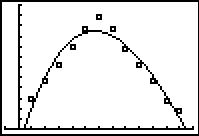
\includegraphics[width=2in]{./PolynomialsGraphics/REG3.jpg} \hspace{.25in} & 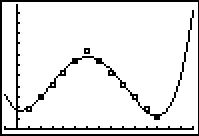
\includegraphics[width=2in]{./PolynomialsGraphics/REG4.jpg} \\

$y = p_{\mbox{\tiny $3$}}(x)$ \hspace{.25in} & $y = p_{\mbox{\tiny $4$}}(x)$ \\

\end{tabular}

\end{center}

\item \begin{enumerate}

\item The scatter plot is shown below with each of the three regression models.

\item The quadratic model is $P_{\mbox{\tiny $2$}}(x) = -0.02x^{2} + 0.241x + 0.956$ with $R^{2} = 0.77708$. \\
The cubic model is $P_{\mbox{\tiny $3$}}(x) = 0.005x^{3} - 0.103x^{2} + 0.602x + 0.573$ with $R^{2} = 0.98153$. \\
The quartic model is $P_{\mbox{\tiny $4$}}(x) = -0.000969x^{4} + 0.0253x^{3} - 0.240x^{2} + 0.944x + 0.330$ with $R^{2} = 0.99929$.

\item The maximums predicted by the three models are $P_{\mbox{\tiny $2$}}(5.737) \approx 1.648$, $P_{\mbox{\tiny $3$}}(4.232) \approx 1.657$ and $P_{\mbox{\tiny $4$}}(3.784) \approx 1.630$, respectively.

\end{enumerate}

\hspace{-.1in} \begin{tabular}{ccc}

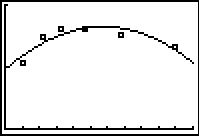
\includegraphics[width=1.8in]{./PolynomialsGraphics/CIRC2.jpg} \hspace{.1in} &
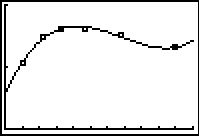
\includegraphics[width=1.8in]{./PolynomialsGraphics/CIRC3.jpg} \hspace{.1in} &
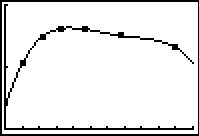
\includegraphics[width=1.8in]{./PolynomialsGraphics/CIRC4.jpg} \\

$y = P_{\mbox{\tiny $2$}}(x)$ \hspace{.1in} & $y = P_{\mbox{\tiny $3$}}(x)$ & $y = P_{\mbox{\tiny $4$}}(x)$\\

\end{tabular}

\end{enumerate}

\closegraphsfile